
The \textbf{behaviours} of non linear systems can be differ a lot from the linear one. The first difference we observed was that while for an LTI system we can say that \textbf{the system is stable} (stability as a property of the system), for non linear systems we talk about \textbf{the stability of a trajectory (or solution)} (stability as a property of a particular solution $x(t)$ of the system). \\
The phenomena which occurs in the case of non linear system are for example: \begin{itemize}
    \setlength\itemsep {0em}
    \item multiple isolated equilibrium points (see the example)
    \item limit cycles
    \item bifurcations
    \item finite escape time
    \item chaos
    \item ...
\end{itemize}

\section{Phase plane portrait}
We focus in this part on \textbf{Second-Order systems}, that are those for which $n_x=2$. The \textbf{phase plane analysis} is a method for studying the properties of such systems, for higher dimensions we can use a sort of generalization represented by the \textit{Poincare Maps}.\\
The analysis we conduct reguard the \textbf{free evolution} of the system, and it is done in order to understand the most intrinsic properties of the system itself.   \\

\noindent
\textbf{Definition} (Phase Portrait, in Italian "Ritratto di fase") Let us consider an \textit{autonomous system} with state $x=(x_1, x_2)\in\mathbb{R}^2$: $\dot{x}(t)=f(x)$, but we can write it also as: 
\begin{align*}
    &\dot{x_1}=f_1(x_1, x_2)   \\
    &\dot{x_2}=f_2(x_1, x_2)
\end{align*}
For any initial condition $x(0)$ the integration of the equation generates a solution and consequently a trajectory. If we repeat the integration for different $x(0)=x_0$ we obtain a family of trajectories which is called {\color{red} \textbf{phase portrait}}.\\

\noindent
\textbf{Example} (Mass-Spring-Damper)\\
Let us consider a \textbf{mass-spring-damper} system with $F=0, \quad \beta=0,\quad m=1,\quad k=1$. The dynamic equation of the system is $\ddot{p}+p=0$, it has solution: $p(t)=p_0 \cos t$ and $\dot{p}(t)=-p_0 \sin t$. We have in this case $x_1=p(t)$ and $x_2=\dot{p(t)}$. \\
We can determine a well known relation between the two variables that we can plot in the \textit{phase plane} or \textit{state domain}. This equation is: $p^2+\dot{p}^2=p_0^2$ which defines a circle of radius $p_0$ in the phase plane. Varying $p_0$ we obtain the \textbf{phase portrait} representation.

\begin{figure}[h]
    \centering
    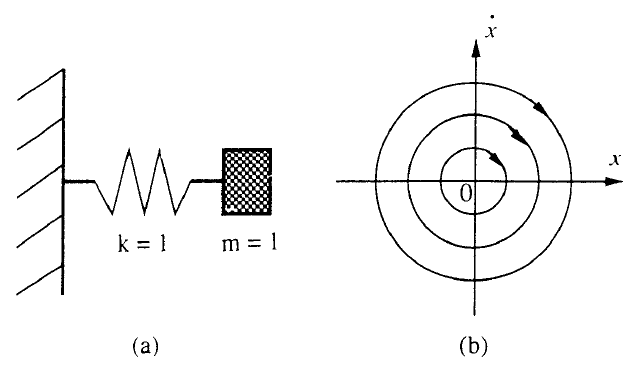
\includegraphics[scale=0.7]{NonLinearControl/images/PhasePort_MSD.png}
    \caption{Mass-Spring-Damper and its \textit{phase portrait}}
    \label{fig:enter-label}
\end{figure}

\subsection{Singular Points} 
Given the system $\dot{x}=f(x)$ with $x \in X \subseteq \mathbb{R}^2$. We define the \textbf{slope} of a trajectory at a point $x=(x_1, x_2)$ as: $$\frac{dx_2}{dx_1}=\frac{f_2(x_1, x_2)}{f_1(x_1, x_2)}$$
At this point we can distinguish \textbf{two cases}: 
\begin{itemize}
    \item $f_2(x_1, x_2)\ne 0, f_1(x_1, x_2)\ne 0$ in this case the slope is \textbf{well defined} and the trajectories won't intersect in the phase plane; 
    \item $f_2(x_1, x_2)=f_1(x_1, x_2)=0$ we can't define the slope that is \textbf{undetermined}, and so some trajectories intersect at point $x=(x_1, x_2)$. We call this point \textbf{singular (or fixed) point}.
\end{itemize}

\noindent
\textbf{Important!} As in the case of the \textit{singular points} we assume that $\dot{x_1}=f_1=0 $ and $\dot{x_2}=f_2=0$ follows that the points for which this happen, are also \textbf{equilibrium points}. They are stable if all trajectory \textbf{converge} to this equilibrium point.

\begin{figure}[h]
    \centering
    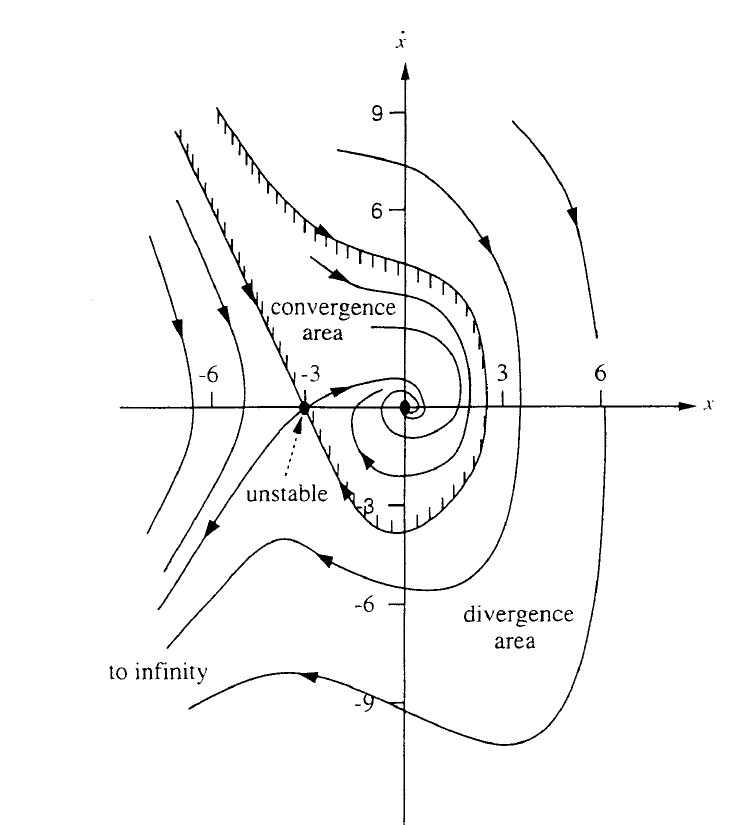
\includegraphics[scale=0.55]{NonLinearControl/images/SingularPoints.png}
    \caption{The phase portrait of a Non Linear System}
    \label{fig:phase}
\end{figure}

\subsubsection{Some considerations}
\begin{itemize}
    \item The Figure \ref{fig:phase} cannot be the phase portrait of an LTI system: in that case we have either one or infinity equilibrium points. This highlight that in the non linear case there can exist few isolated equilibrium points;
    \item In the figure there are two equilibrium point: one is \textit{stable} another is \textit{unstable}.
    \item The figure is the phase portrait linked to the following example:
    \begin{figure}[h]
        \centering
        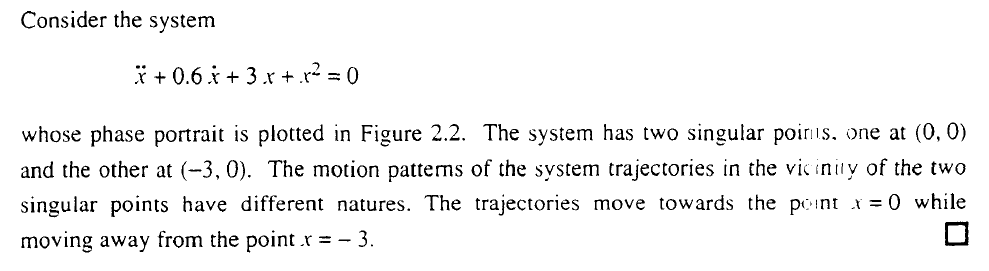
\includegraphics[scale=0.8]{NonLinearControl/images/Slotine1.png}
        \label{fig:enter-label}
    \end{figure}
\end{itemize}

\noindent
It is interesting to note that a phase portrait might by drawn even for a \textbf{first order system}, the difference is that we would have only one trajectory on which we can choose the initial condition. We show here an example (from book "Applied non linear control" - Slotine, 1996): 
\begin{figure}[h]
    \centering
    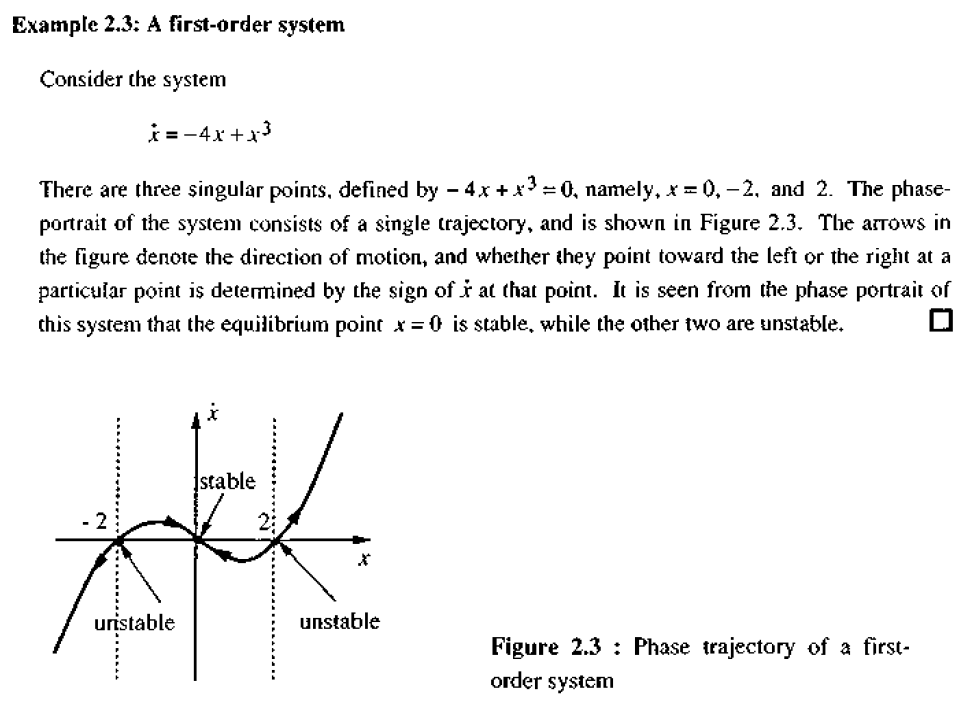
\includegraphics[scale=0.8]{NonLinearControl/images/ExFirstOrder.png}
    \caption{Example of first order phase portrait}
    \label{fig:enter-label}
\end{figure}


\subsection{Methods to draw phase portrait}
There are mainly \textbf{two methods} for constructing the \textit{phase portrait}: 
\begin{enumerate}
    \item \textbf{Analytical/Geometrical methods}: they can be applied only in particular cases; 
    \item By using \textbf{Numerical simulation}: can be applied in any case, moreover they can be generalized to system of order higher than 2.
\end{enumerate}

\section{Behaviour of LTI systems}
Studying the phase portrait of \textbf{LTI systems} is important because: i) we can have an idea of their behaviour, ii) We can use them to study locally the (continuous) non-linearities. We are talking about systems of the form $\dot{x}=Ax$ which have quite simple properties: 
\begin{enumerate}
    \item An LTI system has a \textbf{unique equilibrium point} if the matrix A is non-singular, such point is stable if the eigenvalues of the A matrix have strictly negative real part, \textit{regardless the initial conditions}; 
    \item The solutions can be computed analitically in an easy way; 
    \item In presence of an input $ut(t) \ne 0$ the system becomes of the form $\dot{x(t)}=Ax(t)+Bu(t)$ and we can observe that: 
    \begin{enumerate}
        \item We can apply the \textbf{superposition princple }; 
        \item The asimptotic stability leads to BIBO stability
        \item If $u(t)=A\sin(\omega t + \phi)$, the output is a sinusoidal signal of the same frequency and (Magnitude, Phase) depending on the transfer function of the system itself.
    \end{enumerate}
\end{enumerate}

In order to give consider the case when $A\in \mathbb{R}^{2,2} \quad x \in \mathbb{R}^2$, the system has got \textbf{two eigenvalues} $\lambda_1, \lambda_2$. Actually, we can distinguish the following cases:
\begin{enumerate}
    \item \textbf{$\lambda_{1, 2}$ with the same sign (node)}, if they are both negative, all solution converge otherwise all diverge; 
    \begin{figure}[h]
        \centering
        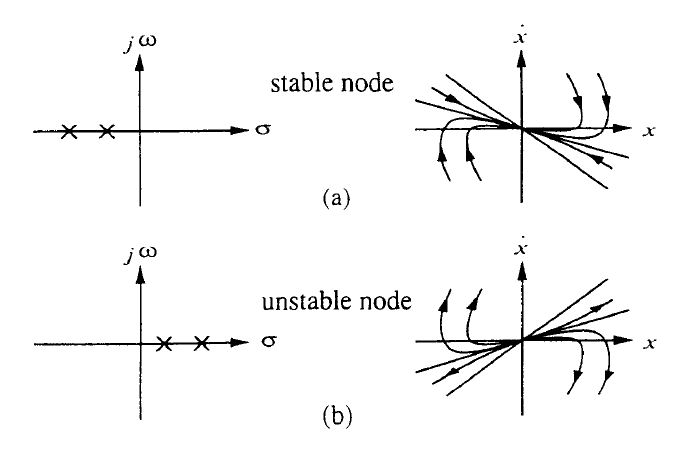
\includegraphics[scale=0.8]{NonLinearControl/images/node.png}
        \caption{Stable/Unstable Node }
        \label{fig:enter-label}
    \end{figure}
    
    %----------------------------------------------
    \item \textbf{$\lambda_{1, 2}$ with opposite signs (saddle)}, in this case as we have some positive, some negative eigenvalue $\Rightarrow$ some solutions converge other diverge; 
    
    \begin{figure}[h]
        \centering
        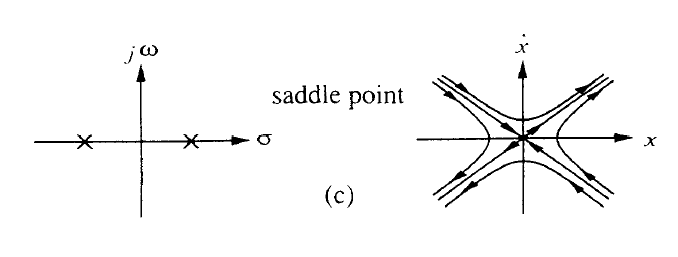
\includegraphics[scale=0.8]{NonLinearControl/images/saddle.png}
        \caption{Saddle point}
        \label{fig:enter-label}
    \end{figure}
     %----------------------------------------------
    \item \textbf{$\lambda_{1, 2}$ complex conjugate with non-zero real part (focus)} in this case if $\textrm{Re}(\lambda_{1,2})<0$ the solutions converge, if $\textrm{Re}(\lambda_{1, 2})>0$, the solutions diverge.
    \begin{figure}[h]
        \centering
        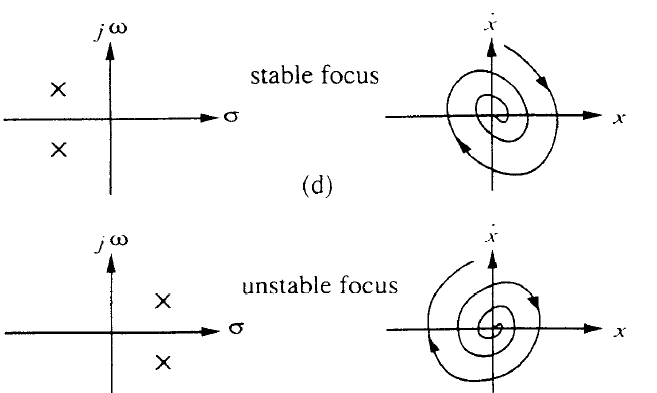
\includegraphics[scale=0.8]{NonLinearControl/images/focus.png}
        \caption{Caption}
        \label{fig:enter-label}
    \end{figure}
    
     %----------------------------------------------
    \item \textbf{$\lambda_{1, 2}$ complex conjugate with zero real part (center)} some  trajectories are \textbf{ellipsis} as they are composition of harmonic signals; 

    \begin{figure}[h]
        \centering
        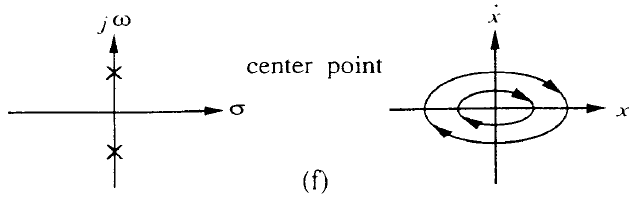
\includegraphics[scale=0.8]{NonLinearControl/images/center.png}
        \caption{Caption}
        \label{fig:enter-label}
    \end{figure}
\end{enumerate}


\section{Non linear case}
The \textbf{behaviour of non linear systems} is much more complex, due to the lack of linearity and superposition principle, they respond to external inputs in a different way. Next we enumerate the most common behaviours: multiple equilibrium points, limit cycles, bifurcations, finite escape time, chaos...

\subsection{Multiple isolated equilibrium points}
Some non linear systems (e.g. the pendulum) have multiple equilibrium points which are isolated, that is in the vicinity there no other equilibrium points. As we said before in the case of LTI systems there only two possibilities: (1) \textbf{a single equilibrium point}, (2) infinitely many equilibrium points in the case that $\textrm{det}(A)=0$.

\subsection{Limit cycles}
A \textbf{limit cycle} is an \textbf{isolated closed curve} on which the motion is \textit{periodic}. A famous example is the \textbf{Van Der Pol oscillator} which is substantially a mass-spring-damper system with a non linear damper.\\
\textit{Limit  cycles} are unique properties of non linear systems, the limit cycle has to be both:
\begin{enumerate}
    \item \textbf{closed}, this feature indicate the periodic motion
    \item \textbf{isolated}, with nearby trajectories that converge or diverge from it.
\end{enumerate}
Depending on the motion of the trajectories in the vicinity of the limit cycle, it can be called:
\begin{itemize}
    \item \textbf{Stable limit cycle}: all trajectories in the "neighbourhood" converge to it $\rightarrow$ we have an \textbf{ATTRACTOR}; 
    \item \textbf{Unstable limit cycle}: all trajectories diverge from the limit cycle $\rightarrow$ we have a \textbf{REPELLOR}; 
    \item \textbf{Semi-Stable limit cycle}: some trajectories converge to it, other diverge $\rightarrow$ we have a \textbf{SADDLE}; 
\end{itemize}

\begin{figure}[h]
    \centering
    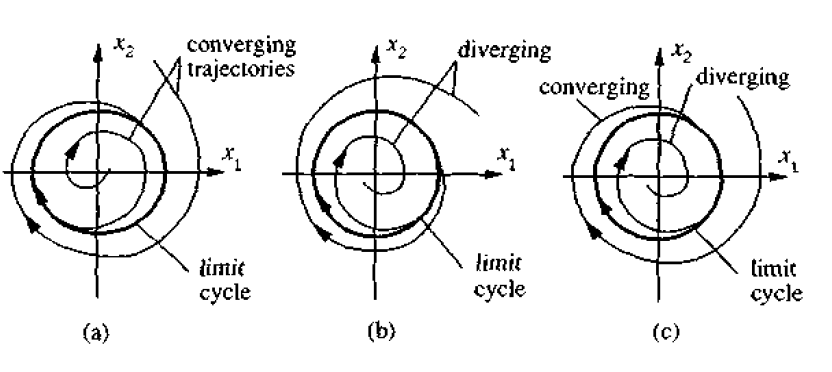
\includegraphics[scale=0.7]{NonLinearControl/images/limitcycles.png}
    \caption{Types of \textbf{limit cycles}}
    \label{fig:enter-label}
\end{figure}
The limit cycle of a \textit{Van Der Pol} oscillator is a stable one.\\
Limit cycles represent an important phenomenon in non linear systems as they can be encountered in many engineering applications and in nature. To give an example in the Aerospace field a limit cycle caused by the interaction between \textit{aerodynamic forces} and \textit{structural vibrations} can be very dangerous. Other times a limit cycle could be desirable! An engineer has to know \textbf{how to eliminate them} when undesirable, how to \textbf{create/amplify} them when they give some advantages. There are some \textbf{simple theorems} that provide a method to individuate them by analyzing some mathematical properties of the system.

\subsubsection{Tori}
When the order of the system is that $n_x>3$, than the motion in the state space can occur on a Torus which constitute a generalization of non-isolated cycle (pendulum) or limit  cycles in \textit{higher dimension}, for this reason, it can be an attractor, repellor or saddle.

\subsection{Bifurcations}
When the \textbf{physical parameters} of a system change, can change also the equilibrium points combined with their stability properties. The values of the parameters ($\alpha$) in general for which this variations occurs are called \textbf{critical} or \textbf{bifurcation values}.\\
The \textbf{bifurcation}, i.e. the \textbf{quantitative change of the parameters} resulting in a \textbf{qualitative change of the system} is another property which characterize non linear systems.\\
Common examples are \textbf{pitchfork} and \textbf{Hopf} bifurcations.

\subsection{Finite escape time}
Is a phenomenon by which some states diverge in a finite time we call $t_esc$, that is equivalent to state that $\lim_{t\to\infty}x(t)=\infty$.

\section {Chaotic systems}
For LTI systems, small differences in initial conditions can cause small differences in the output. For non linear systems is different: there are many cases in which a \textbf{small difference in the initial conditions} is able to lead to \textbf{unpredictable behaviours}, this phenomenon is called \textbf{chaos}. It is useful to distinguish chaos from random motion, in the case of \textit{chaos} the problem is deterministic and there is a small uncertainty in the initial conditions.\\
Chaotic behaviours can be observed in many physical systems (e.g. the \textbf{atmosphere model} can be described like this), the most common is the \textbf{turbulence} in fluid mechanics.\\
In the context of \textbf{feedback control} it  is important to recognize when a system can enter in a chaotic behaviour, and techniques to recover the system itself from it are required.
The motion on these systems can occur over geometric entities with \textbf{fractal structures} called \textbf{strange attractors}, besides you can have \textbf{strange repellors} and \textbf{strange saddles}. Their dimensions are measured by using the \textbf{Housdorff dimensions}. \\

One of the classical \textbf{academic examples} is the \textit{Chua circuit}, which is a quite simple electrical circuit with a non linear resistor whose trajectories are strange attractors. The figure shows two different solutions with different initial conditions.

\begin{figure}[h]
    \centering
    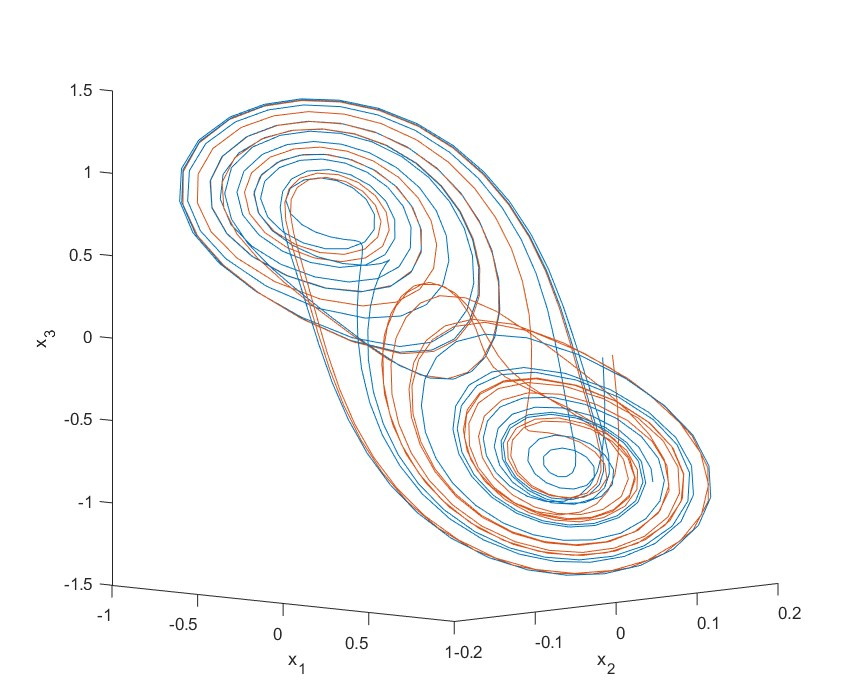
\includegraphics[scale=0.36]{NonLinearControl/images/chuaAttr.jpg}
    \caption{Strange attractor for the \textit{Chua Circuit }}
    \label{fig:enter-label}
\end{figure}

\begin{figure}[h]
    \centering
    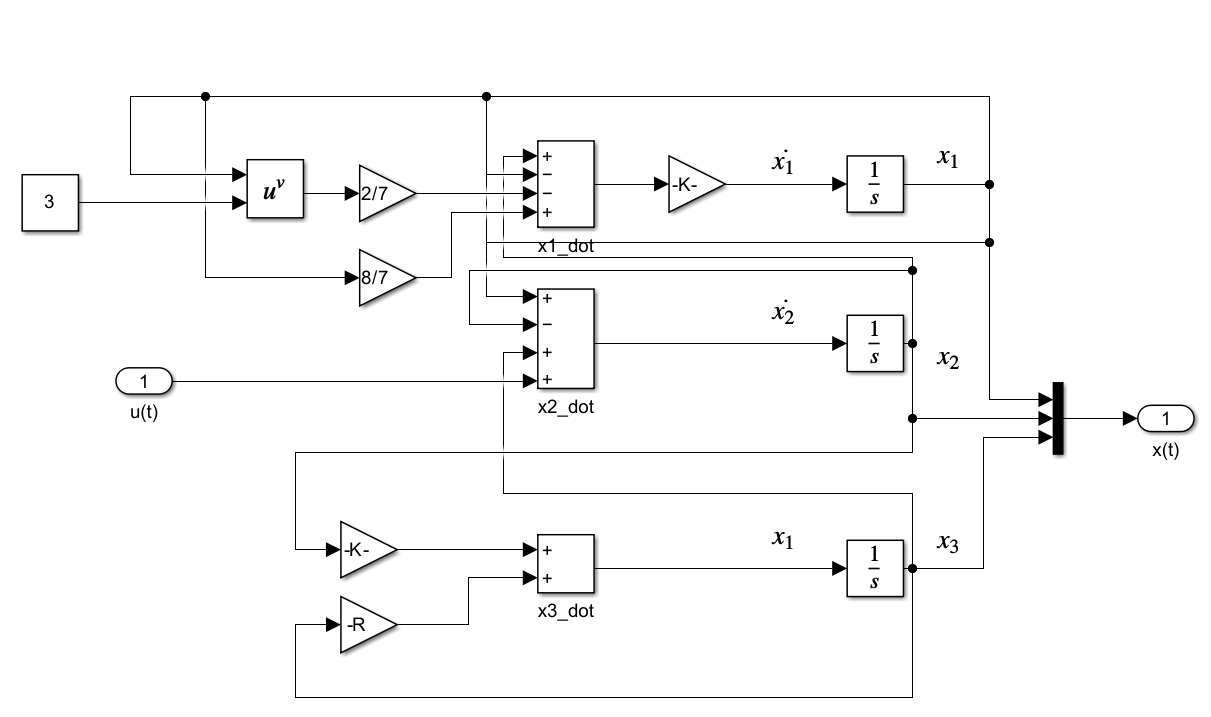
\includegraphics[scale=0.5]{NonLinearControl/images/slk_model.png}
    \caption{Simulink model for the Chua Circuit}
    \label{fig:enter-label}
\end{figure}

